\chapter{Using QTHardMon}

QTHardMon lets you to read in and modify register values of individual boards / cards on your crate. The QtHardMon GUI can list out all registers available for a card along with the current content in these registers. It lets you write custom values to these registers as well (where applicable), thus letting you customize functionality in your cards.

\section{Specifying The Crate Through The .dmap File}
Before the software can be used, the user has to create a .dmap file. The contents of this file lets the software know about the current set of cards plugged in to the crate. Once a correctly written .dmap file is loaded, the software can list out the cards and their internal registers. 

The .dmap file is essentially made up of lines with the following syntax:
\begin{lstlisting}
<card_alias>  <card_device_file_identifier> <path_to_map_file>
\end{lstlisting}

Each such line in the .dmap file describes a card of the crate.
\mbox{\textless card\_alias\textgreater}  is an alternative name the user specifies for the card. The GUI will list the card using this alias name.
\mbox{\textless card\_device\_file\_identifier\textgreater} is the device file identifier of the plugged in card and \mbox{\textless path\_to\_map\_file\textgreater} is the register mapping file for the card. This mapping file is generated by the firmware and contains the list of registers along with their properties such as register size.
	

An example .dmap file could be as below:
\begin{lstlisting}
# filename: example_crate.dmap
card1    /dev/mtcadummys0 ./mtca_card_registers.map
card2    /dev/llrfdummys4 ./llrf_card_registers.map
\end{lstlisting}


The first line beginning with the \# indicates a comment. 

Line 2 and 3 of the \textit{example\_crates.dmap} file indicates that the user wants to configure a crate that has two cards plugged in- \textit{/dev/mtcadummys0} and \textit{/dev/llrfdummys4} (\textit{/dev/mtcadummys0} and \textit{/dev/llrfdummys4} are device file identifiers for these cards).  In our example the alias names for cards represented by \textit{/dev/mtcadummys0} and \textit{/dev/llrfdummys4} are card1 and card2 respectively. Once \textit{example\_crates.dmap} is loaded, the cards will be referred to as card1 and card2 in the GUI.
mtca\_card\_registers.map and llrf\_card\_registers.map are the register mapping files for \textit{/dev/mtcadummys0} and \textit{/dev/llrfdummys4} respectively. 


\section{Loading The Crate Configuration/.dmap File}
Once the cards on your crate have been specified through the .dmap file, the next step is loading this configuration on to the GUI. This is done using the "Load Boards" button on the GUI or using the menu option under \textit{File > Load Boards}: (Fig \ref{load_boards_open_menu_to_load_dmap})

\begin{figure}[htbp]
\centering
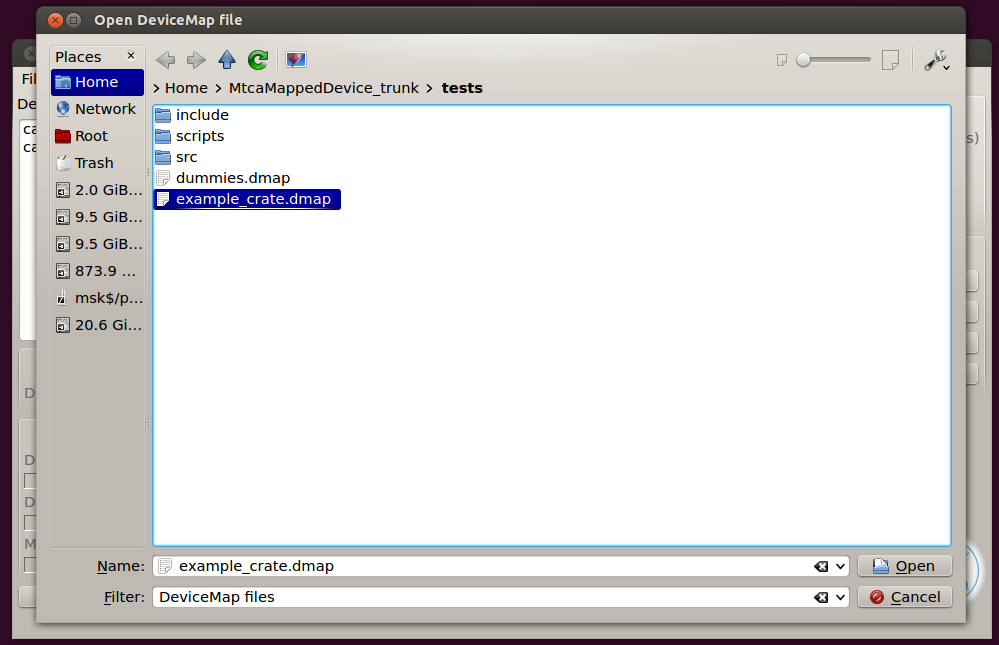
\includegraphics[width=1\textwidth]{images/load_boards_2.png}
 \caption{Loading the .dmap file}
\label{load_boards_open_menu_to_load_dmap}
\end{figure}

\begin{figure}[htbp]
\centering
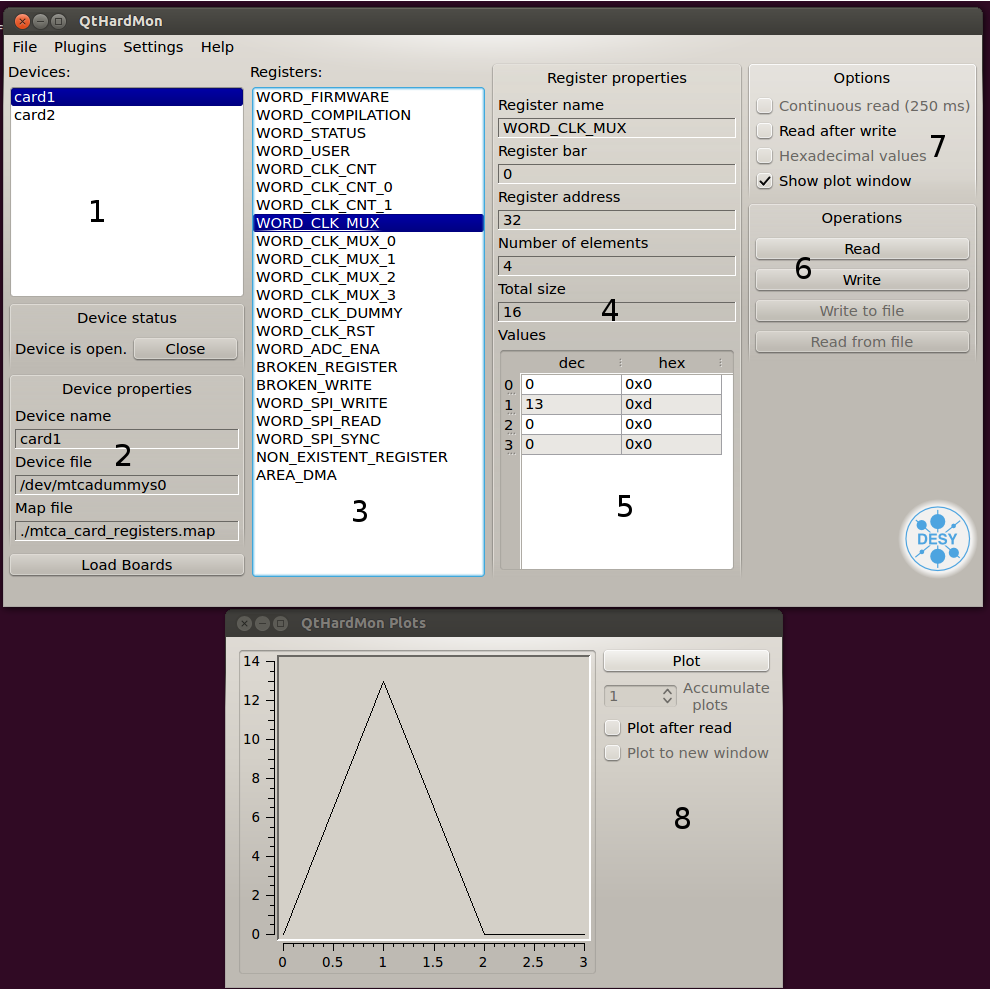
\includegraphics[width=1\textwidth]{images/explain_windows.png}
 \caption{The QtHardMon Interface}
\label{qthardmon_interface}
\end{figure}

\section{The QtHardMon Interface}
Information on the individual cards become available in the GUI once the .dmap is loaded (Fig \ref{qthardmon_interface}). The GUI is split into sections that display information on the cards and these are numbered as in Fig \ref{qthardmon_interface}. The numbered components of the QtHardMon Interface are as below:
\begin{enumerate}
\item \textbf{Devices List:} This section displays the list of cards that were specified in the .dmap file. The user can click on the listed alias names to select individual cards and then modify/display properties of that particular card. 

\item \textbf{Device Status and Properties:} Gives an option to open or close the card selected in the \texttt{Devices List}. The information on the device identifier and register mapping file of this card is also displayed here. Basically all the information on the card from the .dmap file is shown here. 

\item \textbf{Register List:} This part of the GUI displays all registers of the card that are accessible to the user. The GUI can be configured to perform a read on a register when its name is clicked on in the \texttt{Register List}. Successive clicks on the same register name leads to successive reads from the cards, each read corresponding to each click. This behaviour is active, if the \texttt{`Read on click in register list'} check-box is selected in the preferences menu (Section \ref{sub::imp_read}). Selecting the register name using the arrow keys on the keyboard can also trigger a read (in case \texttt{`Automatically read when selecting a register'} is selected in the preferences).

\item \textbf{Register Properties:} The properties of the currently selected register is shown here. These include the register name, the PCI express \textbf{Base Address Range} (Register \textbf{bar}), the register address, the number of 32 bit words in the register and the size of the register in bytes.

\item \textbf{Register Values:} This displays the current value in the register. Both decimal and hexadecimal representations of the value are displayed here. This field is also used to write custom values into the writeable registers of the card. The write to a register is done by setting the intended value in the decimal field and then pressing the write button in the \texttt{Register Operations} section of the GUI.

\item \textbf{Register Operations:} \label{itm:Register_Operations} This part has two working buttons, the first is the \texttt{Read} and the other is the \texttt{Write} button. The default behaviour of the GUI is to read in the register values from the card when the register name is selected or clicked on. The read button is useful when the implicit read functionality has been disabled in the preferences menu(\ref{sub::imp_read}). In this situation the user has to explicitly ask the GUI to perform a read from the card by pressing the \texttt{Read} button.

The \texttt{Write} button is needed because writing to a register using the GUI, is a two step process. The first step is selecting the register on the card and setting the desired value in the \texttt{Register Values} field and the second part is actually triggering the write to the card by pressing the \texttt{Write} button. The value is written only if the \texttt{Write} button is pressed, else it gets discarded when the user moves on to select another register/card or presses the \texttt{Read} button. 

\item \textbf{GUI options:} If the check-box titled \texttt{`Read after Write' is selected}, the GUI actually performs a read from the register and refreshes the display with the new value once the \texttt{Write} button is clicked. The second check-box named \texttt{`Show plot window'} opens a plot display window when checked. The function of this  plot window is explained below.

\item \textbf{Plot Window:} The plot window can be used to draw graphs, using the data contained in the registers. The x-axis of the plot is the number of data points/32 bit elements that has been read in from the register and the y-axis is the value of those elements. It is also possible to customize the number of data points on the x-axis by limiting the number of read in values from the register (See section \ref{subsub::graph_x_axis}).

The GUI by default generates a plot (for the selected register) only after the \texttt{Plot} button is clicked. This default behaviour can be modified by setting the \texttt{`Plot after read'} check-box in the \texttt{Plot Window}. Selecting this option triggers plotting of the register values, once the register name is clicked on or selected using the arrow keys. (Note: This behaviour works as described only when \texttt{`Automatically read when selecting a register'} and \texttt{`Read on click in register list'} options are selected in the preferences menu \ref{sub::imp_read}).
	
%(Note: By default the GUI performs an implicit read of the register values from the card when the register is clicked/selected. This is why the check-box option `Plot after read' plots the register values as soon as the register is selected (basically selecting the register in this case is actually reading its content from the card and hence triggering the plot). A thing to note is that the GUI can be set to disable this implicit read when clicking/selecting the register name. The option to do this is in the preferences menu (see section \ref{preference_section}). If these implicit read options are disabled in the preferences, then selecting the `Plot after read' option will trigger the plot only after the read button or the plot button is clicked.)

\end{enumerate}

%\section{Reading and Writing To a Register}
%See item \ref{itm:Register_Operations} of section \ref{qthardmon_interface}.

\section{The Preferences Menu}\label{preference_section}
The QtHardMon preferences menu can be accessed under \textit{Settings > Preferences} of the main menu. (Fig \ref{qthardmon_preferences})

\begin{figure}[htbp]
\centering
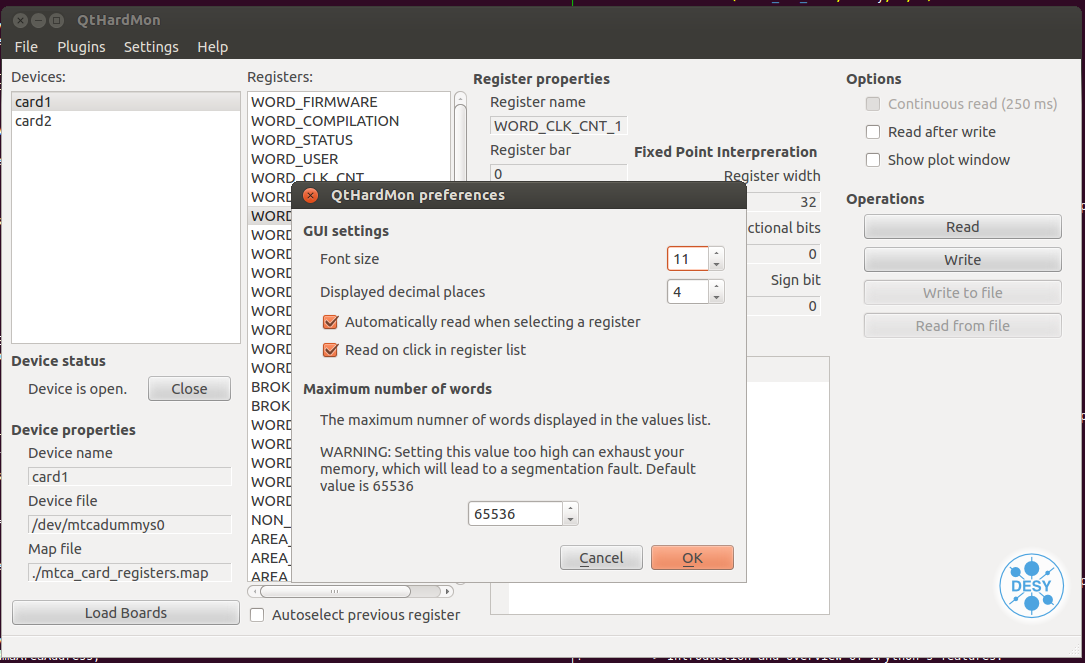
\includegraphics[width=1\textwidth]{images/preferences.png}
 \caption{The QtHardMon Preferences}
\label{qthardmon_preferences}			
\end{figure}

\subsection{Changing The Font Size}
The font size of the GUI can be specified here in the preferences menu, by setting required font size in the provided field.

\subsection{Implicit read of Register Values}\label{sub::imp_read}
The two check-boxes - \texttt{`Automatically read when selecting a register'} and \texttt{`Read on click in register list'} are enabled by default. These options trigger an implicit read of the selected register, as soon as the register name is selected from the Register list using the arrow keys on the keyboard or when the name is clicked on (respectively). These check boxes lets the user disable implicit read when selected or clicked. This is useful in case of large registers, where implicitly reading in these slows down the work flow. The \texttt{Read} button in the \texttt{Register Operations} can be used for reading in values, when both these options are turned off

\subsection{Limiting The Number Of Read In Values}\label{subsub::graph_x_axis}
There can be problems when registers have a large number of elements/32-bit words and when all these words are read in one go. The \texttt{`Maximum number of words'} lets the user limit the number of elements read in from the register. The software reads in only the first `N' elements specified in the \texttt{`Maximum number of words'} field, though the register may contain even more elements. The default value of this field is set as 65536, which means that the maximum number of elements that will be read in from any register is 65536. Setting a higher value here and thus reading in larger amounts of data from a register can potentially exhaust the system memory, leading to a crash.
		
\section{Saving and Restoring Preferences}
As seen, the preferences menu (Section \ref{preference_section}) lets the user customize font size and behaviour of the GUI. The software lets the user save these customizations as a configuration file (.cfg), which can later be loaded back into a fresh session to restore the user defined settings if needed.

The option for saving and loading the GUI configuration file can be found under \textit{File > Save config} / \textit{File > Save config as} and \textit{File > Load config }menu items respectively. The configuration file stores/retrieves the following information:

\begin{itemize}
\item The loaded .dmap file.
\item The selected card/device.
\item The selected registers on all cards.
\item The user selected settings in the prefrences menu
\item The user selected settings in the \texttt{GUI Options}
\item The user selected settings in the \texttt{Plot Window}
\end{itemize}



% info is displayed in three windows as in fig 2 (labelled as 1, 2, 3)
%
%
%dicates tha
%basically it is the list of boards that the user is planning to put into each slot position of the crate. each is mapped to some .map  file.

%configured through a .dmap file 

%
%Load boards
%This software does this and this for you?
%Create a crate config make your changes and get it back later. So u can have different crate configurations that u can build up. Modify register value on the cards and get  stuff done.
%
%Future revisons of the software would like to keep your changes persistent. Why coz u can load up and u r ready to go. Dont have to reprovision stuff again. 
%
%Creating the .dmap file
%format
%dummyname /dev/<name> mapping
%
%the dummyname can be
%
%what would I want from a crate.....
%decide on what cards to put in. - freely let u rearrange?
%%< auto detect what cards are plugged in the crate>
%< freely rearrange the crds >
%< Type of cards>




